\chapter{Conclusions and Future Work}
\label{chapter:conclusion}

This dissertation focuses on using data-driven approaches
to optimize workload and system performance in the cloud.
We study cloud architecture tuning (CAT), which brings great benefits
of cloud computing---tuning architecture for a workload at a time.
Our prototype system \scout consists of
guided search, relative ordering, low-level insights and
transfer learning---enabling
an \emph{efficient}, \emph{effective} and \emph{reliable} CAT method
in an \emph{automatic} and \emph{scalable} way.
This Chapter concludes this dissertation and discuss its future work.

\section{A Practical Guide to Cloud Optimizer}
\label{sec:guide}

%\subsection{Selecting the Right Optimizer}

\iffalse
\begin{figure}[!htbp]
 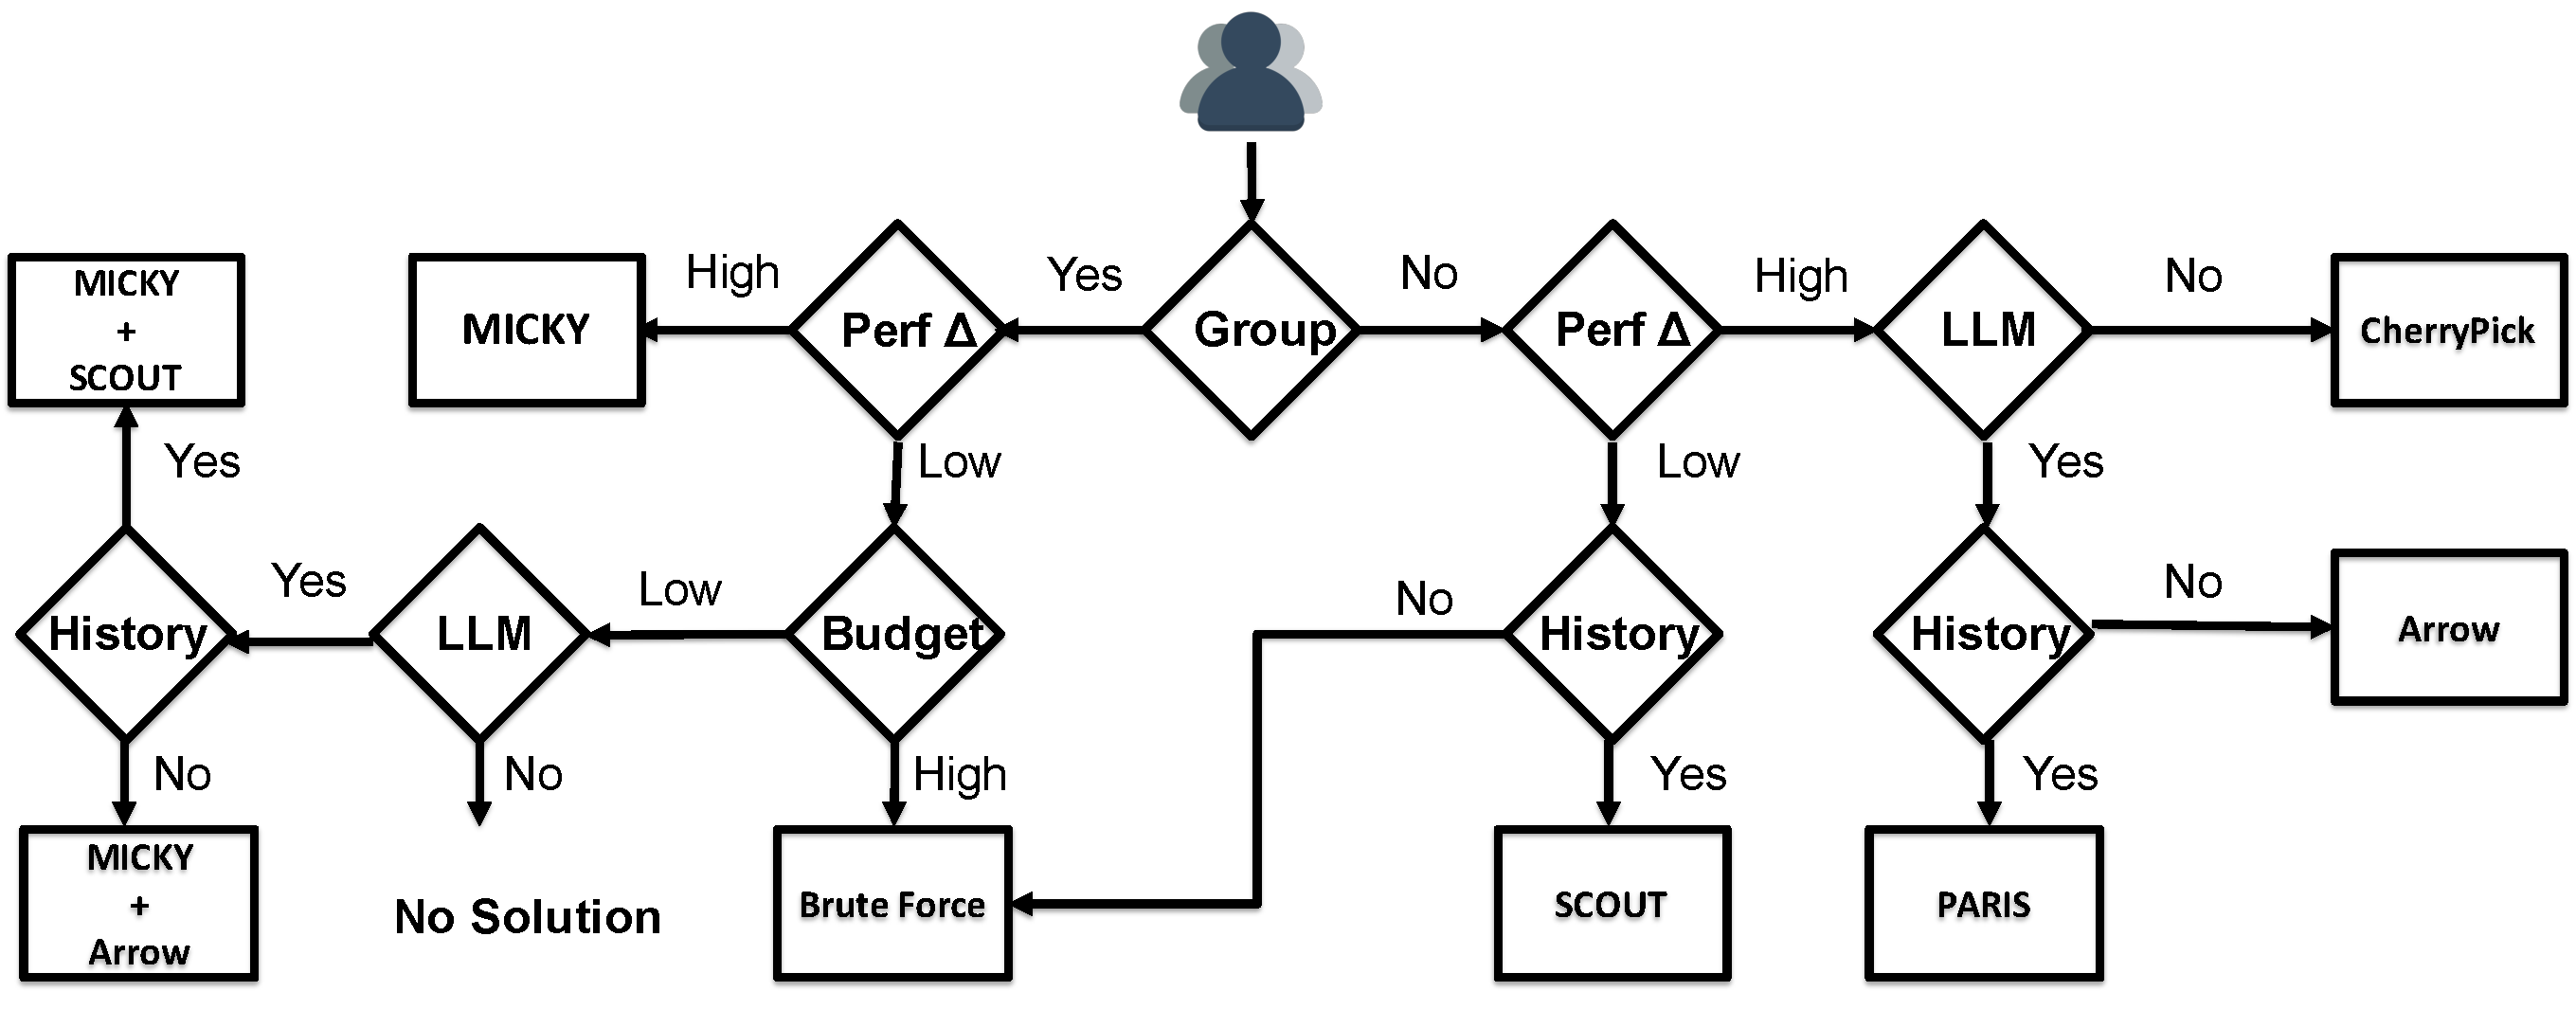
\includegraphics[width=.9\textwidth]{Figures/practical_guide_thesis.pdf}
 \centering
 \caption{\textbf{A practical guide to choosing the right optimization method.} \emph{CheeryPick} works for any workloads without historical and low-level performance data~\cite{Alipourfard2017}. \emph{Arrow} uses low-level metrics to augment Bayesian Optimization (used in \emph{CherryPick})~\cite{Hsu2018Arrow}.  \emph{PARIS} requires low-level and historical data for predicting execution time and running cost of workloads on different VM types~\cite{Yadwadkar2017}.  \scout leverages a learning model and sequential model-based optimization (SMBO) to deliver efficient, effective and reliable recommendation~\cite{Hsu2018Scout}.  \emph{Micky}, different from others, applies collective optimization to largely reduce measurement cost.}
 \label{fig:practical_guide}
\end{figure}
\fi

To pick an optimizer, we should compare its search performance and measurement cost, and understand their assumptions and constraints.
In \mytable{~\ref{tab:cat_guide}}, we derive a practical guide
for selecting an optimizer.
This guide is derived based on extended literature review and our extensive experimentation.

\textbf{Historical data} are execution records of workloads on cloud configurations.
\cherrypick and \arrow do not use historical data (from other workloads) and therefore, require significant initial measurements for 
building prediction models while
\paris and \scout uses historical data.

\textbf{Low-level Metrics} are runtime information (such as CPU utilization, memory usage, and I/O rates) for better characterizing
workloads.
If such low-level information is accessible, users should choose optimizers that leverage low-level performance information.

\textbf{Reliability} 
represents whether a CAT method can deliver consistent search performance and maintain reasonable search cost
across diverse workloads.
Some cloud optimizers may suffer from
the fragility issue or high prediction error.
They are considered less reliable.
When using these optimizers, users should be more careful
because they do not know whether the recommended configurations by the optimizers are near-optimal or sub-optimal.

\iffalse
\textbf{Budget} is the measurement cost a user is willing to pay for an optimizer.
While the brute force approach delivers the best search performance,
it is too expensive in practice.
Using the state-of-the-art methods, for example,
\emph{CherryPick} incurs measurement cost of about 22\% to 33\% of the configuration space, and
\emph{Scout} reduces the cost down to 11\% to 19\% while achieving similar or better search performance~\cite{Hsu2018Scout}.
\fi

In this dissertation, our proposed \scout is \textit{effective}, \textit{efficient} and \textit{reliable}
for any single workload.
On the other hand, we propose a collective optimizer \micky to further reduce search cost while delivering comparable search performance for a group of workloads.
To address the sub-optimal choices in some workloads, we propose an integration with \scout for further optimization.


\begin{table}[ht]
\centering
\caption{\textbf{A practical guide to choosing the right optimization method.} \emph{CheeryPick} works for any workloads without historical and low-level performance data~\cite{Alipourfard2017}. \emph{Arrow} uses low-level metrics to augment Bayesian Optimization (used in \emph{CherryPick})~\cite{Hsu2018Arrow}.  \emph{PARIS} requires low-level and historical data for predicting execution time and running cost of workloads on different VM types~\cite{Yadwadkar2017}.  \scout leverages a learning model and sequential model-based optimization (SMBO) to deliver efficient, effective and reliable recommendation~\cite{Hsu2018Scout}.  \emph{Micky}, different from others, applies collective optimization to largely reduce measurement cost.
}
\resizebox{\columnwidth}{!}{%
\begin{tabular}{ clccc}
\toprule
	\textbf{CAT Optimizer} & \textbf{Solution} & \textbf{Historical Data} & \textbf{Low-Level Metrics} &  \textbf{Reliability} \\
\midrule
	\multirow{6}{*}{Single} & CherryPick~\cite{Alipourfard2017} & \xmark & \xmark & \xmark \\
     & Brute Force & \xmark & \xmark & \cmark \\
	 & Arrow~\cite{Hsu2018Arrow} & \xmark & \cmark & \cmark \\
	 %& No Proposed Solution & \cmark & \xmark & \cmark \\
	 & PARIS~\cite{Yadwadkar2017} & \cmark & \cmark & \xmark \\
	 & SCOUT~\cite{Hsu2018Scout} & \cmark & \cmark & \cmark \\
\midrule
	\multirow{4}{*}{Collective} & Micky~\cite{Hsu2018Micky} & \xmark & \xmark & \xmark \\
	 %& No Proposed Solution & \xmark & \xmark & \cmark \\
	 & Micky + Arrow & \xmark & \cmark & \cmark \\
	 & Micky + Scout~\cite{Hsu2018Micky} & \cmark & \cmark & \cmark \\
\bottomrule
\end{tabular}
}
\label{tab:cat_guide}
\end{table}


\section{Conclusion}

\begin{itemize}

\item Low-level performance information is essential to
characterize workloads predict systems performance.
With low-level performance insights, we are able to understand
workload behavior and system behavior
without expert knowledge---not to mention the increasing complexity in
software systems and applications.
%With this line to research,
%we can expect a broad spectrum of performance optimization proposed
%for many evolving applications in the cloud.

\item
Although machine learning tools are readily available,
off-the-shelf methods are far from ideal.
For better predicting workload and system performance,
we need to avoid generalization error.
We propose leveraging low-level performance information to
improve generalization capability.
We also design a two-level learning method that
reduces the overfitting problem.

\item
Bayesian Optimization is a powerful device
for optimizing any black-box functions---well suited to CAT problem.
However, high-level features---such as core counts, memory size,
and cluster sizes---are not sufficient to accurately predict performance.
Our novel optimization method alleviates the fragility issue
by embedding low-level performance insights.
Together with relative ordering and transfer learning, we can
find near-optimal architectural choices with only a handful of trials.

\item
When a cluster is resized to reflect the workload changes,
we need to optimize data placement to release the full capacity of
the resized cluster.
We find that workload-aware data placement with fine-grained partitioning
better balances the loads and tolerates mispredictions of loads.

\end{itemize}

\section{Future Work}

This dissertation has shown that data-driven approaches are very promising
to optimize system performance.
To further improve this line of research,
we should focus on building accurate prediction models and
understanding the relationship between architecture, workload, and performance.

\begin{itemize}

\item \textbf{Synthetic performance data.}
The efficacy of data-driven approaches relies on quality data.
A key element to quality data is to ensure that comprehensive workloads
are included in the performance data.
However, data collection from real-world applications is difficult
to guarantee such comprehensiveness.
In this dissertation, we assume we have obtained comprehensive data
by using a large set of diverse workloads.
However, it is impossible to claim to have comprehensive data
unless we can define the whole spectrum of workload behavior.
To solve this problem, we should be able to generate performance data
using synthetic program that simulates comprehensive workload behavior
such as CPU-intensive, memory-intensive and I/O-intensive.
With the synthetic program, we can control the ratio of
computation, memory access, and I/O characteristics.
Training a prediction model with comprehensive performance data will
improve prediction quality.


\item \textbf{Performance extrapolation.}
Generalizing performance behavior beyond the training data is very difficult.
This dissertation does not examine performance extrapolation---when
the target cluster size is several times larger.
This is particularly important, for example, to accelerate
big data analytics jobs.
\ernest exploits workload and system knowledge
for building accurate prediction models~\cite{Venkataraman2016}.
However, Ernest is very expensive because it requires separate training
processes for different workloads and different virtual machine types.
We believe that low-level performance insights and comprehensive synthetic performance data
might help extrapolate scaling behavior better.

%\item \textbf{Fine-grained tuning.}
%Our proposed methods are built for ``sparse'' discrete search space.


\end{itemize}

Performance optimization is a long-standing research problem.
This dissertation examines several challenges of
applying machine learning techniques to
optimizing system performance in the cloud.
As cloud computing becomes more prominent,
hosted applications become more complex, and
architectural choices become more customizable,
data-driven approaches---due to
its black-box feature and its prediction capability---will be
a vital device to optimize workload and system performance in cloud computing.
